\documentclass[border=6pt]{standalone}
\usepackage{tikz}
\usetikzlibrary{arrows.meta,positioning,calc,shapes.geometric,fit,backgrounds,patterns,matrix,decorations.pathreplacing}
\begin{document}
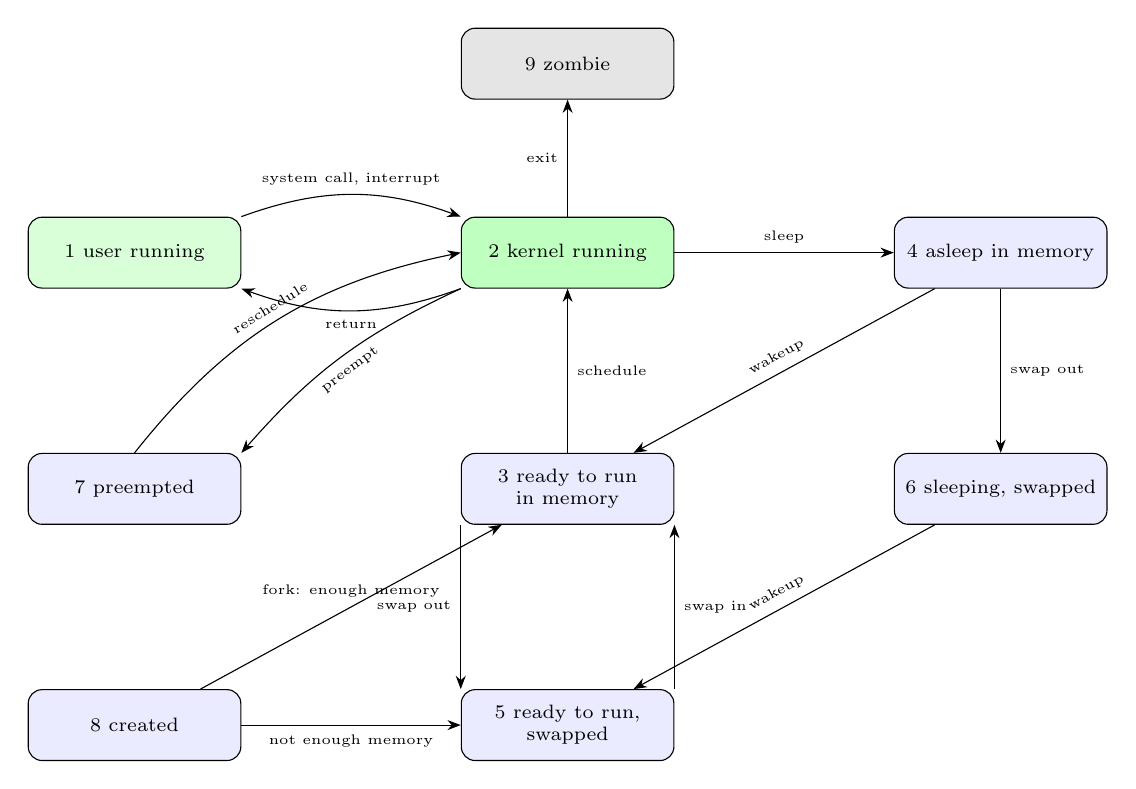
\begin{tikzpicture}[>=Stealth,font=\small]
\tikzstyle{st}=[draw,rounded corners=5pt,minimum width=2.7cm,minimum height=0.9cm,fill=blue!8,font=\scriptsize,align=center]
\node[st,fill=green!15] (1) at (0,0) {1 user running};
\node[st,fill=green!25] (2) at (5.5,0) {2 kernel running};
\node[st,fill=gray!20] (9) at (5.5,2.4) {9 zombie};
\node[st] (4) at (11,0) {4 asleep in memory};
\node[st] (7) at (0,-3) {7 preempted};
\node[st] (3) at (5.5,-3) {3 ready to run\\ in memory};
\node[st] (6) at (11,-3) {6 sleeping, swapped};
\node[st] (8) at (0,-6) {8 created};
\node[st] (5) at (5.5,-6) {5 ready to run,\\ swapped};
\draw[->] (1.north east) to[bend left=20] node[above,font=\tiny]{system call, interrupt} (2.north west);
\draw[->] (2.south west) to[bend left=20] node[below,font=\tiny]{return} (1.south east);
\draw[->] (2) -- node[left,font=\tiny]{exit} (9);
\draw[->] (2) -- node[above,font=\tiny]{sleep} (4);
\draw[->] (4) -- node[right,font=\tiny]{swap out} (6);
\draw[->] (4) -- node[above,font=\tiny,sloped]{wakeup} (3);
\draw[->] (2.south west) to[bend right=12] node[below,font=\tiny,sloped]{preempt} (7.north east);
\draw[->] (7.north) to[bend left=20] node[above,font=\tiny,sloped]{reschedule} (2.west);
\draw[->] (3) -- node[right,font=\tiny]{schedule} (2);
\draw[->] (3.south west) -- node[left,font=\tiny]{swap out} (5.north west);
\draw[->] (5.north east) -- node[right,font=\tiny]{swap in} (3.south east);
\draw[->] (6) -- node[above,font=\tiny,sloped]{wakeup} (5);
\draw[->] (8) -- node[above,font=\tiny]{fork: enough memory} (3);
\draw[->] (8) -- node[below,font=\tiny]{not enough memory} (5);
\end{tikzpicture}
\end{document}
